Habiendo abordado el funcionamiento de los agentes especialistas en el Capítulo 6, este capítulo se centra en los mecanismos de coordinación que permiten la operación del sistema completo.

Para ello se introducirá la lógica del agente planificador, el agente orquestador y el agente principal (MainAgent). Posteriormente se detallarán las variaciones exploradas en dicho marco de coordinación.

\section{Agente Principal}
\label{sec:principal}
Este agente define la lógica de enrutación entre el planificador y el orquestador, introduciendo finalmente el resultado al agente formateador. 

Para ello, primero se ejecuta el agente planificador, el cual genera un plan a alto nivel consistiendo de varios pasos a ejecutar. Tras esto se ejecuta el agente orquestador con el primer paso del plan generado, el cual tendrá que decidir cuales agentes especializados ejecutar para dicho paso. Los agentes seleccionados serán ejecutados de forma asíncrona, generando cada uno un \opus{CitedAIMessage}, constituido por el contenido de la respuesta y una lista de Citas para los documentos utilizados en la respuesta.

Se ejecutan iteraciones de dicho proceso hasta que el planificador determina que el plan ha finalizado. Tras esto, el agente formateador estructura la respuesta en un formato de respuesta. Este constituye un mensaje markdown y la lista de indentificadores para las citas a referenciar.  

Dado que se han desarrollado varias versiones de planificadores y orquestadores, para poder realizar las variaciones detalladas en la Sección \ref{sec:vars} se ha implementado un patrón Builder para construir el sistema apartir de los agentes indicados. El Listado \ref{lst:builder} ilustra la creación, inicialización y ejecución del sistema mínimo con los cinco agentes especialistas. 

\begin{lstlisting}[caption={Instanciación y ejecución del sistema mínimo con el patrón Builder},label={lst:builder}]
  builder = FlexibleAgentBuilder()
  agent = await (await (builder
                 .reset()
                 .with_main_agent_type("basic")
                 .with_planner_type("basic")
                 .with_orchestrator_type("basic")
                 .with_specialized_agents([
                      CodeAgent(),
                      CachedConfluenceAgent(),
                      GitlabAgent(),
                      FileSystemAgent(),
                      GoogleDriveAgent(),
                  ])
                 .initialize_agents())).build()

  result = await agent.execute_agent_graph_with_exception_handling({
      "query": "Qué entornos de despliegue existen en el proyecto?",
  })
\end{lstlisting}

El Listado \ref{lst:structured_output} muestra la ejecución de un modelo con salida estructurada para poder interpretar su salida desde un entorno de código. El adaptador \opus{with_structured_output} añade una explicación al prompt del mdoelo que indica cuál es el esquema JSON a utilizar como salida. Posteriormente esta salida de serializa a un objeto de Python. El código ilustra varios intentos en caso de no recibir un objeto correctamente estructurado, utilizando para ello un \opus{RetryOutputParser} de LangChain, el cual intenta que otro LLM genere la estructura requerida partiendo de la respuesta anterior. 
\todo{No sé donde meter esto}

\begin{lstlisting}[caption={Validación de la salida estructurada de un LLM},label={lst:structured_output}]
  async def execute_structured_llm_with_validator_handling(prompt: str | Sequence[BaseMessage], output_schema: Type[BaseModel], max_retries: int, llm: BaseChatModel) -> BaseModel:

    structured_model = llm.with_structured_output(output_schema)
    parser = PydanticOutputParser(pydantic_object=output_schema)
    retry_parser = RetryOutputParser.from_llm(parser=parser, llm=default_llm)

    for _ in range(max_retries):
        try:
            response = await structured_model.ainvoke(prompt)
            raw_response = response if isinstance(response, str) else None
            # Si no sigue la estructura intentar convertirla directamente 
            if not isinstance(response, output_schema):
                response = output_schema.model_validate(response)

        except Exception as e:
          # Si no se convierte intentar parsear la respuesta con otro LLM  
          response = retry_parser.parse(raw_response)
        ...

        return response
\end{lstlisting}

\section{Agente Planificador}

Este agente crea planes de alto nivel para estructurar el proceso de respuesta en un procedimiento lógico. Adicionalmente, el agente debe modificar dinámicamente los planes en base al estado de ejecución actual.

El agente sigue el flujo ilustrado en la Figura \ref{fig:planner}. Inicialmente se verifica que el plan no esté finalizado mediante el condicional \opus{check_current_plan()}. Se considera que el plan está finalizado si la ejecución del planificador anterior así lo ha marcado o se ha superado el límite de iteraciones establecido.

\begin{figure}[h]
  \centering
  \adjustbox{center=\textwidth}{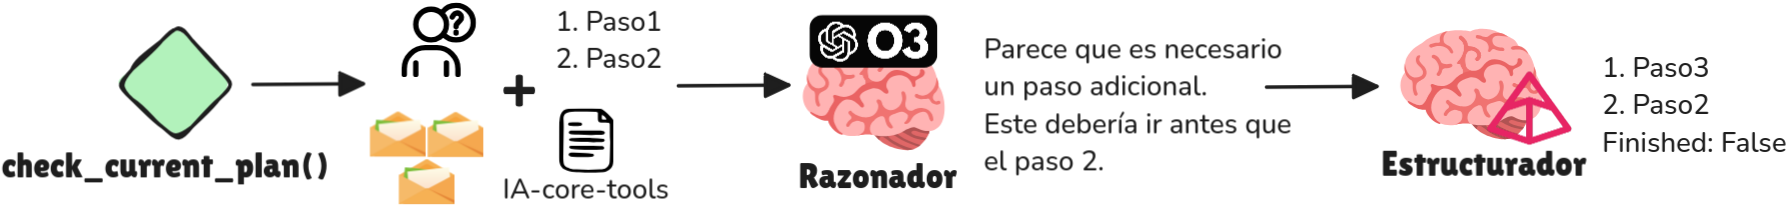
\includegraphics[width=1.25\linewidth]{figures/planner.png}}
  \caption{Flujo de ejecución del agente planificador}
  \label{fig:planner}
\end{figure}
Después, un agente razonador recibe la consulta del usuario y una descripción breve del proyecto. En caso de no ser la primera iteración para la ejecución, este recibe también el plan anterior y las respuestas de los agentes especializados, los cuales representan el resultado de ejecución del primer paso del plan anterior. Este agente deberá razonar sobre los pasos siguientes a realizar, generando un plan nuevo o modificando el actual. 

Finalmente, otro agente estructura el plan textual del razonador a un modelo de Pydantic, que consiste en un objeto de python representado en una lista de pasos textuales con un argumento booleano que indica si el plan ha finalizado. El razonador no estructura su plan porque los agentes razonadores han sido ajustados para devolver una respuesta sin un formato establecido, e indicarle el formato a utilizar ha demostrado reducir la precisión del razonamiento.


\section{Agente orquestador}
Este agente recoge una tarea a realizar, ya sea un paso de un plan o una pregunta directamente, y decide cuáles agentes ejecutar de forma asíncrona.

Para fundamentar su respuesta, se incluye en su prompt una descripción de cada agente disponible, con un breve resumen del tipo de información que contiene cada uno. Este prompt se construye dinámicamente en base a los agentes disponibles, guardando dicha descripción en la clase \opus{SpecializedAgent}. 

\section{Variaciones de orquestación}
\label{sec:vars}
El sistema base sigue la descripción de la sección \ref{sec:principal}, donde un orquestador selecciona los agentes a ejecutar para los pasos del plan generados por un planificador. En cambio, en un enfoque diferente se ha explorado la posibilidad de  







Explicar esto paso por paso.
Por ejemplo, si el usuario pregunta por ejemplos en los que se utiliza la guía de estilos del proyecto, un primer paso expresaría la necesidad de localizar la guía de estilos, para en un segundo paso buscar implementaciones específicas en el código fuente.
